\documentclass[a4paper,landscape]{article}

\usepackage[margin=7mm]{geometry}
\usepackage{mathtools}
\usepackage{fontspec}
\usepackage{unicode-math}
\setmainfont{DejaVu Sans}
\setsansfont{DejaVu Sans}
\setmathfont{Latin Modern Math}[Scale=MatchUppercase]

\usepackage[final]{microtype}
\usepackage{tabularx,array}
\usepackage{ragged2e}
\usepackage{xcolor}
\usepackage{tikz}
\usetikzlibrary{calc,positioning}
\usepackage{pgfplots}
\pgfplotsset{compat=1.18}
\usepackage[most]{tcolorbox}

\definecolor{Ink}{HTML}{17212B}
\definecolor{Teal}{HTML}{147D7E}
\definecolor{TealSoft}{HTML}{DDEEEE}
\definecolor{Coral}{HTML}{E36B55}
\definecolor{Gold}{HTML}{D6A442}
\definecolor{Mist}{HTML}{F1F4F3}
\definecolor{Paper}{HTML}{FBFCFA}
\definecolor{Rule}{HTML}{CBD5D2}
\definecolor{Muted}{HTML}{5C6B73}
\definecolor{White}{HTML}{FFFFFF}

\pagestyle{empty}
\setlength{\parindent}{0pt}
\setlength{\parskip}{0pt}
\setlength{\tabcolsep}{3.5pt}
\setlength{\abovedisplayskip}{3.4pt}
\setlength{\belowdisplayskip}{3.4pt}
\setlength{\abovedisplayshortskip}{2pt}
\setlength{\belowdisplayshortskip}{2pt}
\setlength{\jot}{1.6pt}
\renewcommand{\arraystretch}{1.16}

\newcommand{\term}[1]{\textcolor{Teal}{\bfseries #1}}
\newcommand{\warn}[1]{\textcolor{Coral}{\bfseries #1}}
\newcommand{\muted}[1]{\textcolor{Muted}{#1}}
\newcommand{\divider}{\par\vspace{1.25mm}{\color{Rule}\hrule height .3pt}\vspace{1.25mm}}
\newcommand{\stepchip}[1]{%
  \tikz[baseline=(n.base)]\node[
    inner xsep=1.6mm,inner ysep=.55mm,rounded corners=1.1mm,
    fill=TealSoft,text=Teal,
    font=\fontsize{6.3}{6.7}\selectfont\bfseries
  ](n){#1};%
}

\newtcolorbox{plotcard}[2][]{%
  enhanced,
  height=64mm,
  colback=Paper,
  colframe=Rule,
  colbacktitle=Paper,
  coltitle=Ink,
  boxrule=.4pt,
  arc=2.3mm,
  outer arc=2.3mm,
  boxsep=0pt,
  left=2.2mm,right=2.2mm,top=.9mm,bottom=1.4mm,
  toptitle=.9mm,bottomtitle=.7mm,
  titlerule=.32pt,
  title={%
    \fontsize{9.1}{9.5}\selectfont\bfseries\MakeUppercase{#2}%
  },
  borderline west={1.35pt}{0pt}{Teal},
  #1
}

\newtcolorbox{infocard}[3][]{%
  enhanced,
  height=77mm,
  colback=Paper,
  colframe=Rule,
  colbacktitle=Paper,
  coltitle=Ink,
  boxrule=.4pt,
  arc=2.3mm,
  outer arc=2.3mm,
  boxsep=0pt,
  left=2.8mm,right=2.8mm,top=1.7mm,bottom=1.8mm,
  toptitle=1mm,bottomtitle=.8mm,
  titlerule=.32pt,
  title={%
    \textcolor{Coral}{\fontsize{6.4}{6.7}\selectfont\bfseries #2}%
    \hspace{1.5mm}%
    \fontsize{9.2}{9.7}\selectfont\bfseries\MakeUppercase{#3}%
  },
  borderline west={1.35pt}{0pt}{Teal},
  #1
}

\newtcolorbox{formula}[1][]{%
  enhanced,
  colback=TealSoft!65!Paper,
  colframe=TealSoft,
  boxrule=.3pt,
  arc=1.6mm,
  boxsep=0pt,
  left=1.7mm,right=1.7mm,top=1.2mm,bottom=1.2mm,
  before skip=.5mm,after skip=1.4mm,
  #1
}

\pgfplotsset{
  visualplot/.style={
    width=.90\linewidth,
    height=44mm,
    scale only axis,
    axis lines=middle,
    axis line style={draw=Muted!75,line width=.4pt},
    ticklabel style={font=\fontsize{5.8}{6.1}\selectfont,text=Muted},
    label style={font=\fontsize{6.2}{6.5}\selectfont,text=Ink},
    grid=major,
    major grid style={Rule!62,line width=.25pt},
    every axis plot/.append style={line width=1.3pt},
    samples=120,
    clip=true
  }
}

\begin{document}
\pagecolor{Mist}
\fontsize{8.25}{9.75}\selectfont
\color{Ink}

\begin{tcolorbox}[
  enhanced,
  height=14.5mm,
  colback=Ink,
  colframe=Ink,
  boxrule=0pt,
  arc=2.7mm,
  outer arc=2.7mm,
  boxsep=0pt,
  left=4.3mm,right=4.3mm,top=1.2mm,bottom=1.2mm,
  before skip=0pt,after skip=2mm,
  overlay={
    \fill[Coral] ([xshift=-18mm]frame.north east) rectangle
      ([xshift=-14.5mm]frame.south east);
    \fill[Gold] ([xshift=-11.7mm]frame.north east) rectangle
      ([xshift=-9.5mm]frame.south east);
  }
]
  \begin{minipage}[c][10.5mm][c]{.84\linewidth}
    {\color{White}\fontsize{19.5}{19.5}\selectfont\bfseries
      EXPONENTS \textcolor{Coral}{\(\leftrightarrow\)} LOGARITHMS}
  \end{minipage}
\end{tcolorbox}

\newcommand{\plotsrow}{%
\noindent
\begin{minipage}[t]{.3225\textwidth}
\vspace{0pt}
\begin{plotcard}{Inverse pair}
  \centering
  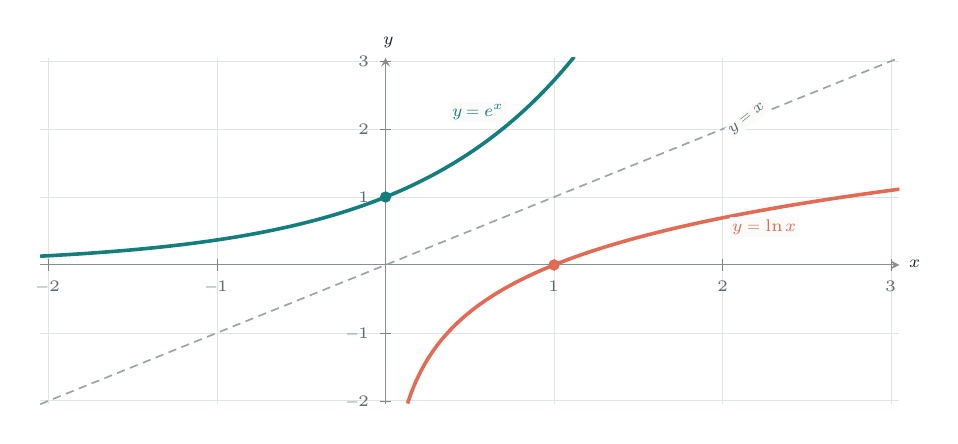
\begin{tikzpicture}
    \begin{axis}[
      visualplot,
      xmin=-2.05,xmax=3.05,
      ymin=-2.05,ymax=3.05,
      xtick={-2,-1,1,2,3},
      ytick={-2,-1,1,2,3},
      xlabel={\(x\)},ylabel={\(y\)},
      xlabel style={at={(axis description cs:1,.405)},anchor=west},
      ylabel style={at={(axis description cs:.405,1)},anchor=south}
    ]
      \addplot[domain=-2.05:1.12,Teal] {exp(x)};
      \addplot[domain=.13:3.05,Coral] {ln(x)};
      \addplot[domain=-2.05:3.05,Muted!62,densely dashed,line width=.6pt] {x};
      \addplot[only marks,mark=*,mark size=1.35pt,Teal] coordinates {(0,1)};
      \addplot[only marks,mark=*,mark size=1.35pt,Coral] coordinates {(1,0)};
      \node[font=\fontsize{6.1}{6.4}\selectfont\bfseries,text=Teal,
        fill=Paper,inner sep=1pt] at (axis cs:.55,2.25) {\(y=e^x\)};
      \node[font=\fontsize{6.1}{6.4}\selectfont\bfseries,text=Coral,
        fill=Paper,inner sep=1pt] at (axis cs:2.25,.56) {\(y=\ln x\)};
      \node[font=\fontsize{5.6}{5.9}\selectfont,text=Muted,rotate=39,
        fill=Paper,inner sep=.8pt] at (axis cs:2.15,2.15) {\(y=x\)};
    \end{axis}
  \end{tikzpicture}
  \par\vspace{.9mm}
  {\fontsize{6.85}{7.45}\selectfont
    Mirror across \(y=x\); \((0,1)\leftrightarrow(1,0)\); asymptotes swap.\par}
\end{plotcard}
\end{minipage}\hfill
\begin{minipage}[t]{.3225\textwidth}
\vspace{0pt}
\begin{plotcard}{The base controls direction}
  \centering
  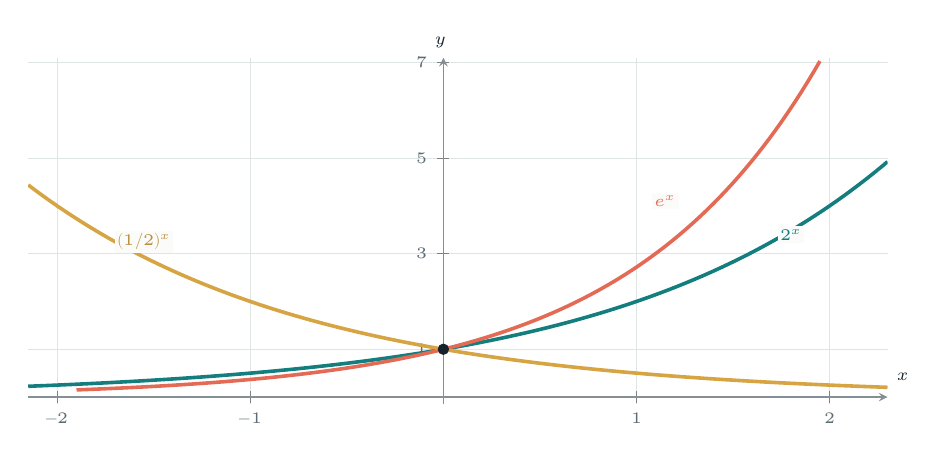
\begin{tikzpicture}
    \begin{axis}[
      visualplot,
      xmin=-2.15,xmax=2.3,
      ymin=-.15,ymax=7.1,
      xtick={-2,-1,1,2},
      ytick={1,3,5,7},
      xlabel={\(x\)},ylabel={\(y\)},
      xlabel style={at={(axis description cs:1,.08)},anchor=west},
      ylabel style={at={(axis description cs:.48,1)},anchor=south}
    ]
      \addplot[domain=-2.15:2.3,Teal] {2^x};
      \addplot[domain=-1.9:1.95,Coral] {exp(x)};
      \addplot[domain=-2.15:2.3,Gold] {.5^x};
      \addplot[only marks,mark=*,mark size=1.35pt,Ink] coordinates {(0,1)};
      \node[font=\fontsize{5.9}{6.2}\selectfont\bfseries,text=Coral,
        fill=Paper,inner sep=1pt] at (axis cs:1.15,4.1) {\(e^x\)};
      \node[font=\fontsize{5.9}{6.2}\selectfont\bfseries,text=Teal,
        fill=Paper,inner sep=1pt] at (axis cs:1.8,3.4) {\(2^x\)};
      \node[font=\fontsize{5.9}{6.2}\selectfont\bfseries,text=Gold!85!Ink,
        fill=Paper,inner sep=1pt] at (axis cs:-1.55,3.25) {\((1/2)^x\)};
    \end{axis}
  \end{tikzpicture}
  \par\vspace{.9mm}
  {\fontsize{6.85}{7.45}\selectfont
    \(a>1\) rises; \(0<a<1\) decays. Every \(a^x\) passes through \((0,1)\).\par}
\end{plotcard}
\end{minipage}\hfill
\begin{minipage}[t]{.3225\textwidth}
\vspace{0pt}
\begin{plotcard}{Growth fingerprints}
  \centering
  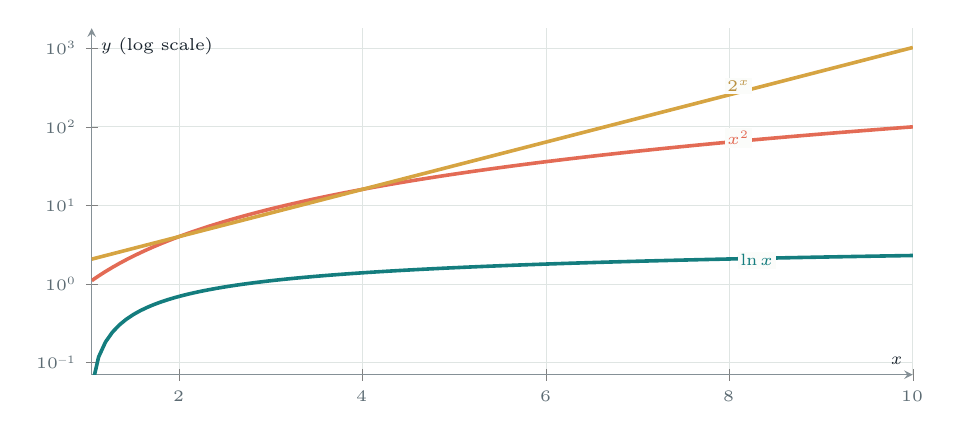
\begin{tikzpicture}
    \begin{axis}[
      visualplot,
      width=.86\linewidth,
      axis lines=left,
      xmin=1.05,xmax=10,
      ymin=.07,ymax=1800,
      ymode=log,
      log basis y=10,
      xtick={2,4,6,8,10},
      ytick={.1,1,10,100,1000},
      xlabel={\(x\)},ylabel={\(y\) (log scale)},
      legend style={draw=none,fill=none}
    ]
      \addplot[domain=1.05:10,Teal] {ln(x)};
      \addplot[domain=1.05:10,Coral] {x^2};
      \addplot[domain=1.05:10,Gold] {2^x};
      \node[font=\fontsize{5.9}{6.2}\selectfont\bfseries,text=Teal,
        fill=Paper,inner sep=1pt] at (axis cs:8.3,2.0) {\(\ln x\)};
      \node[font=\fontsize{5.9}{6.2}\selectfont\bfseries,text=Coral,
        fill=Paper,inner sep=1pt] at (axis cs:8.1,72) {\(x^2\)};
      \node[font=\fontsize{5.9}{6.2}\selectfont\bfseries,text=Gold!85!Ink,
        fill=Paper,inner sep=1pt] at (axis cs:8.1,330) {\(2^x\)};
    \end{axis}
  \end{tikzpicture}
  \par\vspace{.9mm}
  {\fontsize{6.85}{7.45}\selectfont
    On a log-\(y\) scale, exponentials straighten; powers and logs remain curved.\par}
\end{plotcard}
\end{minipage}%
}

\vspace{2mm}

\noindent
\begin{minipage}[t]{.3225\textwidth}
\vspace{0pt}
\begin{infocard}{01}{Core dictionary}
  \begin{formula}
    \centering
    \(\displaystyle
      a^x=e^{x\ln a},\qquad
      \log_a x=\frac{\ln x}{\ln a}
    \)
    \par\vspace{.7mm}
    \(\displaystyle y=a^x \Longleftrightarrow x=\log_a y\)
  \end{formula}
  \vspace{1.4mm}

  \begin{minipage}[t]{.48\linewidth}
    \term{Exponent laws}
    \[
      a^{m+n}=a^ma^n
    \]
    \[
      a^{m-n}=\frac{a^m}{a^n},
      \qquad a^{-n}=\frac1{a^n}
    \]
    \[
      (a^m)^n=a^{mn},
      \qquad (ab)^n = a^nb^n
    \]
  \end{minipage}\hfill
  \begin{minipage}[t]{.48\linewidth}
    \term{Log laws}
    \[
      \log_a(xy)=\log_a x+\log_a y
    \]
    \[
      \log_a(x/y)=\log_a x-\log_a y
    \]
    \[
      \log_a(x^r)=r\log_a x
    \]
  \end{minipage}

  \vspace{4.2mm}
  \divider
  \term{Real-domain assumptions.}
  \(a>0,\ a\neq1\); every logarithm argument is \(>0\).
  Negative bases do not support arbitrary real exponents.

  \vspace{5mm}
  \term{Anchors.}
  \(a^0=1,\ \log_a1=0,\ \log_a a=1\).
\end{infocard}
\end{minipage}\hfill
\begin{minipage}[t]{.3225\textwidth}
\vspace{0pt}
\begin{infocard}{02}{Solving patterns}
  \centering
  \stepchip{DOMAIN}\hspace{.7mm}
  \(\rightarrow\)\hspace{.7mm}
  \stepchip{ISOLATE}\hspace{.7mm}
  \(\rightarrow\)\hspace{.7mm}
  \stepchip{INVERT}\hspace{.7mm}
  \(\rightarrow\)\hspace{.7mm}
  \stepchip{CHECK}
  \par\vspace{2.1mm}
  \RaggedRight

  \begin{tabularx}{\linewidth}{@{}>{\(\displaystyle}l<{\)} X@{}}
    a^{f(x)}=b
      & \(f(x)=\log_a b\), requiring \(b>0\)\\[1mm]
    \log_a f(x)=c
      & \(f(x)=a^c\), then enforce \(f(x)>0\)\\[1mm]
    be^{kx}=c
      & \(x=k^{-1}\ln(c/b)\), requiring \(c/b>0\)\\[1mm]
    xe^x=q
      & \(x=W_k(q)\), with a domain-appropriate branch
  \end{tabularx}

  \vspace{1.3mm}
  \divider
  \term{Example}
  \[
    2^{3x-1}=7
    \quad\Longrightarrow\quad
    x=\frac{1+\log_2 7}{3}.
  \]

  \vspace{1.4mm}
  \term{Lambert \(W\).}
  \(W(z)e^{W(z)}=z\). On the reals,
  \(W_0\) exists for \(z\ge-1/e\), while \(W_{-1}\) supplies a second
  real branch on \([-1/e,0)\).
  \vspace{1.4mm}
  \[
    x^x=c,\ x>0
    \quad\Longrightarrow\quad
    x=e^{W_k(\ln c)}.
  \]
\end{infocard}
\end{minipage}\hfill
\begin{minipage}[t]{.3225\textwidth}
\vspace{0pt}
\begin{infocard}{03}{Models and computation}
  \term{Straight-line tests}
  \[
    y=Ce^{kx}
    \quad\Longleftrightarrow\quad
    \ln y=\ln C+kx
    \qquad\text{(semi-log)}
  \]
  \[
    y=Cx^p
    \quad\Longleftrightarrow\quad
    \ln y=\ln C+p\ln x
    \qquad\text{(log-log)}
  \]
  The slope estimates \(k\) or \(p\); a log transform also changes the
  noise model.

  \vspace{1.4mm}
  \divider
  \term{Stable primitives}
  \[
    \operatorname{log1p}(x)=\ln(1+x),\qquad
    \operatorname{expm1}(x)=e^x-1
  \]
  preserve precision near \(x=0\).

  \vspace{1.3mm}
  \[
    m=\max_i x_i,\qquad
    \operatorname{LSE}(x)
    =m+\ln\sum_i e^{x_i-m},
  \]
  \[
    m\le\operatorname{LSE}(x)\le m+\ln n.
  \]
  \vspace{1.2mm}
  \term{Scale units.}
  \(\log_2\): bits; \(\ln\): nats; \(\log_{10}\): decades.
\end{infocard}
\end{minipage}

\vspace{2mm}

\begin{tcolorbox}[
  enhanced,
  height=28mm,
  colback=Ink,
  colframe=Ink,
  boxrule=0pt,
  arc=2.3mm,
  outer arc=2.3mm,
  boxsep=0pt,
  left=3.2mm,right=3.2mm,top=1.8mm,bottom=1.8mm,
  overlay={
    \draw[White!18,line width=.35pt]
      ([xshift=96mm,yshift=3mm]frame.south west) --
      ([xshift=96mm,yshift=-3mm]frame.north west);
    \draw[White!18,line width=.35pt]
      ([xshift=159mm,yshift=3mm]frame.south west) --
      ([xshift=159mm,yshift=-3mm]frame.north west);
    \draw[White!18,line width=.35pt]
      ([xshift=222mm,yshift=3mm]frame.south west) --
      ([xshift=222mm,yshift=-3mm]frame.north west);
  }
]
  \begin{minipage}[c][22mm][c]{.1\linewidth}
    {\color{Coral}\fontsize{6.3}{6.6}\selectfont\bfseries 04}
    \par\vspace{.5mm}
    {\color{White}\fontsize{10.2}{10.5}\selectfont\bfseries FAST\\CHECKS}
  \end{minipage}\hfill
  \begin{minipage}[c][22mm][c]{.23\linewidth}
    {\color{TealSoft}\bfseries DOMAINS FIRST}
    \par\vspace{.8mm}
    {\color{White!78}
      \(a>0,\ a\neq1\); \\
      log arguments \(>0\);\\
      real exponential outputs are positive.}
  \end{minipage}\hfill
  \begin{minipage}[c][22mm][c]{.21\linewidth}
    {\color{TealSoft}\bfseries FALSE FRIENDS}
    \par\vspace{.8mm}
    {\color{White!78}
      \(\ln(x+y)\neq\ln x+\ln y\);\\
      \((x+y)^r\neq x^r+y^r\) in general.}
  \end{minipage}\hfill
  \begin{minipage}[c][22mm][c]{.20\linewidth}
    {\color{TealSoft}\bfseries TANGENT BOUNDS}
    \par\vspace{.8mm}
    {\color{White!78}
      \(e^t\ge1+t\), \\\(\ln x\le x-1\), \\
      \(\frac{x}{1+x}\le\ln(1+x)\le x\).}
  \end{minipage}\hfill
  \begin{minipage}[c][22mm][c]{.20\linewidth}
    {\color{TealSoft}\bfseries EVENTUAL ORDER}
    \par\vspace{.8mm}
    {\color{White!78}
      \((\ln x)^m\ll x^p\ll a^x\ll\Gamma(x+1)\)
      \\for \(m,p>0,\ a>1\).}
  \end{minipage}
\end{tcolorbox}

\vspace{2mm}
\plotsrow

\end{document}
